\documentclass[main.tex]{subfiles}
\begin{document}

\section{Argument Structure}
\setcounter{section}{6}
%\setcounter{table}{0}
%\setcounter{figure}{0}

\subsection{Verbal Arguments}

In general, every verb in English takes one or more arguments, with a subject argument being required in normal speech and writing. The Stanford NLP system marks the arguments of verbs using the dependencies \textit{ccomp} (clausal complement), \textit{csubj} (clausal subject), \textit{csubjpass} (passive clausal subject), \textit{dobj} (direct object), \textit{iobj} (indirect object), \textit{nsubj} (nominal subject), \textit{nsubjpass} (passive nominal subject), and \textit{xcomp} (open clausal complement). In the majority of non-copular clauses, the governors of these dependencies are the core verbs. In copular sentences, the governor is generally the subject complement (i.e. the argument generally appearing after the verb which is equated with the subject), though in the case of copular sentences with clausal subjects, the Stanford Parser chooses the copula to be the governor.
Examples of these dependencies can be seen in the following sentences taken from the ICE-CAN and MICUSP corpora and from \citet{typed-deps-manual}:
\newline\newline%\begin{tabular}{ l l }
%ICE Canada
\noindent a.{\hskip 1em}\xytext{
\xybarnode{In} &
\xybarnode{nineteen} &
\xybarnode{ninety-seven} &
\xybarnode{Roland} &
\xybarnode{Lemon} &
\xybarnode{was} &
\xybarnode{elected} 
\xybarconnect(U,U){-2}"_{\small nsubjpass}"
\xybarconnect(D,D){1}"_{\small dobj}"
&
\xybarnode{president.} 
}\\
%MICUSP native
\noindent b.{\hskip 1em}\xytext{
\xybarnode{\ldots} &
\xybarnode{before} &
\xybarnode{his} &
\xybarnode{father} &
\xybarnode{gave} 
\xybarconnect(UL,U){-1}"_{\small nsubj}"
\xybarconnect(UR,U){1}"^{\small iobj}"
\xybarconnect(D,D){3}"_{\small dobj}"&
\xybarnode{him} &
\xybarnode{the} &
\xybarnode{rest} &
\xybarnode{of} &
\xybarnode{it.}
}\\
%MICUSP native
\noindent c.{\hskip 1em}\xytext{
\xybarnode{They} &
\xybarnode{state} 
\xybarconnect(U,U){-1}"_{\small nsubj}"
\xybarconnect(D,D){3}"_{\small ccomp}"&
\xybarnode{that} &
\xybarnode{climate} &
\xybarnode{generally} &
\xybarnode{predicts} 
\xybarconnect(U,U){-2}"_{\small nsubj}"
\xybarconnect(D,D){4}"_{\small ccomp}"&
\xybarnode{that} &
\xybarnode{temperatures} &
\xybarnode{should} &
\xybarnode{rise}
\ldots
}\\

%MICUSP native
\noindent d.{\hskip 1em}\xytext{
\xybarnode{Before} &
\xybarnode{Yeltsin} &
\xybarnode{appointed} 
\xybarconnect(U,U){-1}"_{\small nsubj}"
\xybarconnect(D,D){5}"_{\small xcomp}"&
\xybarnode{him} &
\xybarnode{the} &
\xybarnode{deputy} &
\xybarnode{Prime} &
\xybarnode{Minister}
\xybarconnect(U,U){-4}"_{\small nsubj}"&
\ldots
}\\

%Dep Manual
\noindent e.{\hskip 1em}\xytext{
\xybarnode{That} &
\xybarnode{she} &
\xybarnode{lied} 
\xybarconnect(U,U){-1}"_{\small nsubj}"&
\xybarnode{was} &
\xybarnode{suspected}
\xybarconnect(D,D){-2}"^{\small csubjpass}"&
\xybarnode{by} &
\xybarnode{everyone.}
}\\
%Dep manual
\noindent f.{\hskip 1em}\xytext{
\xybarnode{What} &
\xybarnode{she} &
\xybarnode{said} 
\xybarconnect(U,U){-1}"_{\small nsubj}"&
\xybarnode{is} &
\xybarnode{not}&
\xybarnode{true.}
\xybarconnect(D,D){-3}"^{\small csubj}"&
} \newline

%\end{tabular}
%\caption[Examples of the Dependencies Listed in Table~\ref{table:arg-deps}]{Examples of the Dependencies Listed in Table~\ref{table:arg-deps}. \textit{a}, Native Sample from ICE-CAN; \textit{b,c,d}, Native Samples from MICUSP; \textit{e,f} from \citet{typed-deps-manual}.}
%\label{ex:arg-deps}
%\end{figure}

\citet{dubois:2003} provides hints that verbal argument structure may differ between native and nonnative speakers. That study explores when speakers use lexical NPs rather than pronominal NPs as verbal arguments. Considering only native speakers but looking at a number of different languages, Du Bois finds that there is a very strong tendency for speakers to use no more than one lexical argument per finite clause (Du Bois's One Lexical Argument Constraint) and to avoid placing an argument in the subject role of transitive sentences (the Non-Lexical \textbf{A} Constraint\footnote{\citet{dubois:2003} uses the letters \textbf{A}, \textbf{I}, and \textbf{O} to refer to the subject, indirect object, and direct object arguments of a transitive verb, and \textbf{S} to refer to the sole argument of an intransitive verb.}). He makes the case that these rules hold true for a number of world languages. However, in presenting data to show that several languages abide by the Non-Lexical \textbf{A} Constraint, he also shows that there are large differences between languages in the likelihood of a new argument appearing in the direct object and intransitive subject roles \citep[Table~2.5]{dubois:2003}. A new argument is one presenting information that has not yet been presented in the discourse. A new argument generally cannot be a pronoun, as pronouns typically refer to something presented earlier in the discourse. Not all lexical arguments are new arguments of course, but it stands to reason that the factors affecting the ratio of new to old arguments will also affect the ratio of lexical to pronominal arguments. The data he gathers show that in English, on average, 21\% of new arguments are found in intransitive clauses, versus 28\% for Spanish, and 79\% are found in direct object roles, versus 71\% for Spanish. A $\chi^2$ analysis shows that these differences are statistically significant considering his sample sizes ($\chi^2=2.244, df=2, p=0.326$), though admittedly at a relatively low confidence level (70\%). As an aside, of the five languages for which data is presented in that table, English and Spanish are the most similar in new argument distribution. The three other languages considered, French, Hebrew, and Sakapultek, all show a greater probability of finding a new argument in the intransitive subject role, and a lower probability of finding one in the direct object role, than either Spanish or English. Seeing that there may be differences between Spanish and English in how new arguments are distributed among the various argument roles, and noting that other languages show such differences as well, it is worth investigating whether L1-Spanish learners of English differ in their usage of lexical arguments as compared to native speakers.

To investigate the feasibility of classifying language based on argument structure, Stanford dependency graphs were analyzed to identify 18 different types of finite clauses: intransitives with and without clausal subjects, copular clauses with and without clausal subjects, simple transitives with and without clausal subjects and objects, ditransitives with and without clausal subjects, complex transitives with and without clausal subjects, passives of simple transitives with or without clausal subjects, and passives of complex transitives with or without clausal subjects and complements. Then, for each of these 18 different types of clauses, all possible combinations of lexical and non-lexical arguments were considered, yielding 80 different attributes in total. This system, while providing a generous amount of data for the classifiers, yielded decision trees that were difficult to interpret linguistically. Fortunately, it was possible to generate from these attributes three much smaller and more coherent sets of attributes which, when combined and used to train a classifier, provided comparable accuracy.

The first of these attribute sets consisted of just three attributes, each corresponding to a particular verb valency (i.e. the number of arguments). The values associated with these attributes were the percentage of all clauses which used that number of arguments. The next attribute set consisted of four attributes, named \textit{zero, one, two, three}, with corresponding values indicating what percentage of finite clauses had that number of lexical arguments. To avoid lengthy periphrasis, it is convenient to call this metric \textit{lexical argument density}.  The last attribute set consisted of seven attributes corresponding to types of argument roles. The values associated with these attributes were the percentage of lexical arguments found in that type of argument role. The seven types were intransitive, transitive, passive, and copular subjects, indirect and direct objects, and subject complements. This latter category included both the complement of copular clauses and what is usually the third argument in a complex transitive (e.g. \textit{Before Yeltsin appointed him \underline{the deputy Prime Minister}}). This set of attributes will be referred to as the \textit{lexical argument role} set.

To determine what was a lexical argument and what was not, the pronouns \textit{other, another, else, same, one, this, that, these, those, what, myself, yourself, herself, himself, itself, ourselves, yourselves, themselves, oneself, mine, yours, hers, his, ours, theirs, me, you, her, him, it, us, them, I, she, he, we}, and \textit{they} were compared with each argument, and if no match was found, the argument was considered lexical. By this standard, clausal arguments were always considered lexical arguments. 

\begin{comment}
\begin{table}[ht]
\small
\centering
\caption{Pronouns Used to Determine Non-Lexical Status of Arguments}
\begin{tabular}{ l l l l l l l l }
\toprule

other & another & else & same & one \\
this & that & these & those & what \\
myself & yourself & herself & himself & itself \\
ourselves & yourselves &themselves & oneself \\
mine & yours & hers & his & ours & theirs \\
me & you & her & him & it & us \\
them & I & she & he & we & they \\

\bottomrule
\end{tabular}
\label{table:pronouns}
\end{table}
\end{comment}

Figure~\ref{fig:c4.5-val} shows a C4.5 decision tree trained on cases consisting of the three verb valency attributes. It is noteworthy that the tree considers only two of the three attributes, and appears to indicate that native English has a larger proportion of trivalent verbs than does nonnative English, and that the opposite is true of divalent verbs. However, an extremely large number of training cases are misclassified by this tree, particularly by the middle leaf. In fact, Table~\ref{table:val-results} shows that the tree on average only classifies slightly more than half of all test cases correctly, and, worse still, the confidence interval for that accuracy encompasses 50\%, indicating that the tree may be doing no better than a random classifier. It is a bit surprising that the C4.5 algorithm was unable to construct a useful decision tree, as Du Bois presents data showing that there are statistically significant differences in the usage frequency of transitive and intransitive verbs between English and Spanish \citep[Table~2.3]{dubois:2003}. He found that in English 58\% of finite verbs were intransitive and 42\% transitive, whereas in Spanish the numbers were 63\% and 37\%. Furthermore, calculating from the data he gives, this difference is statistically significant at a high level of confidence: $\chi^2=4.693, df=1, p<0.05$. Based on Du Bois's data, one might expect a decision tree to classify texts as native based on a low ratio of transitive (di- and trivalent) verbs to intransitive (monovalent) verbs. However, there are a number of possible reasons why this is not the case, the most obvious being that perhaps this characteristic is not involved in L1-transfer.


\begin{figure}[ht]
\centering
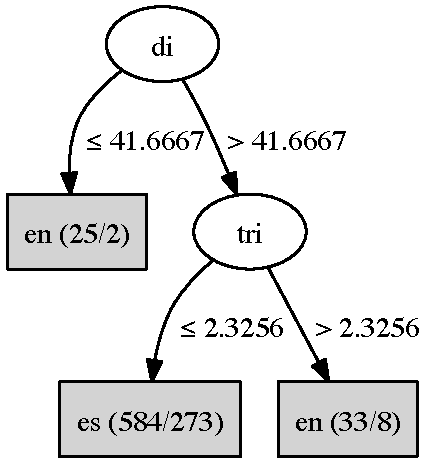
\includegraphics[width=2.1in]{c45-val.pdf}
\caption{Verbal Clause Valency C4.5 Decision Tree}
\label{fig:c4.5-val}
\end{figure}

\begin{table}[ht]
\centering
\caption{Accuracy of Verbal Clause Valency C4.5 Classifier}
\begin{tabular}{l c c}
\toprule
& Mean & 95\% C.I.\\
\midrule
Nonnative & 84.4\% & - \\
[6pt]Native & 17.4\% & - \\
[6pt]Overall & 50.9\% & 47.1\% --- 54.8\% \\
\bottomrule
\end{tabular}
\label{table:val-results}
\end{table}

Figure~\ref{fig:c4.5-num-lex} shows a decision tree generated by the C4.5 algorithm using cases with attributes indicating lexical argument density. Though \citet{dubois:2003} did gather lexical argument density data, he only appears to have done so for English and the Mayan language Sakapultek. The differences between those two languages in this regard are pronounced, but suggest little about any such differences between English and Spanish. The tree itself is unusual, as it considers only two of the four attributes, one of which is considered twice. The first node in the tree checks whether fewer than 8\% of clauses have no lexical arguments and, if so, immediately classifies that case as native. Du Bois's data shows that such clauses are common in spoken English, accounting for a startling 87\% of all clauses. In written English, they are decidedly less common. In the 321 native training cases, finite verbs with no lexical arguments account for only 17\% of all verbs. There does not seem to be much available research on lexical argument density in nonnative language, but it might be conjectured that learners of English have not developed clear distinctions between the written and spoken registers, and thus tend to show some speech-like elements in their written language, such as a high incidence of finite verbs without lexical arguments. 
\begin{figure}[htbp]
\centering
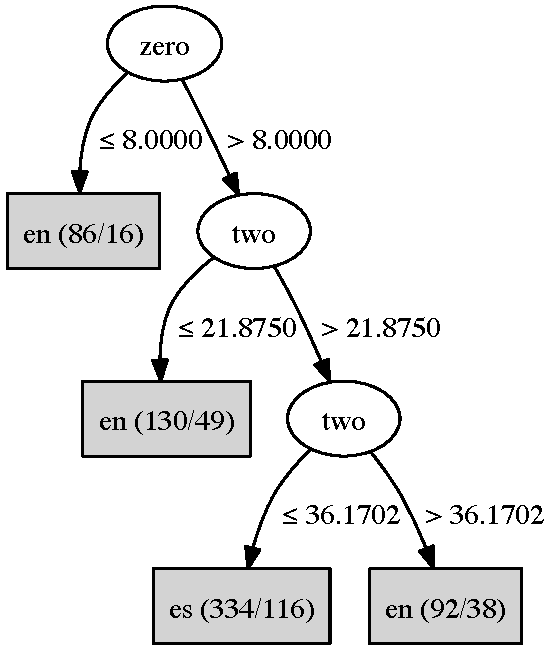
\includegraphics[width=2in]{c45-num-lex.pdf}
\caption{Lexical Argument Density C4.5 Decision Tree}
\label{fig:c4.5-num-lex}
\end{figure}

The other two nodes in Figure~\ref{fig:c4.5-num-lex} are more opaque to interpretation. These nodes both consider the two-lexical-argument attribute, essentially performing a ternary test on it, classifying cases with intermediate values as nonnative and cases with high and low values as native. It is hard to imagine that there is a convincing linguistic reason behind this, particularly considering the high rater of error associated with these nodes. Table~\ref{table:num-lex-results} shows the accuracy of this classification system. As the confidence interval shows, it is an improvement over the valency system, though is still error-prone.

\FloatBarrier
\begin{table}[ht]
\centering
\caption{Accuracy of Lexical Argument Density C4.5 Classifier}
\begin{tabular}{l c c}
\toprule
& Mean & 95\% C.I.\\
\midrule
Nonnative & 70.7\% & - \\
[6pt]Native & 48.6\% & - \\
[6pt]Overall & 58.7\% & 55.9\% --- 63.5\% \\
\bottomrule
\end{tabular}
\label{table:num-lex-results}
\end{table}

Training a C4.5 classifier on the lexical argument role attribute set yields the decision tree shown in Figure~\ref{fig:c4.5-lex-role}. This tree is considerably more complicated than those shown in Figures~\ref{fig:c4.5-val} and \ref{fig:c4.5-num-lex}, and is more accurate, as well. Table~\ref{table:lex-role-results} shows that it correctly classifies test cases approximately two thirds of the time. Considering this tree in light of Du Bois's data shows some interesting parallels. Of the three roles that he considered, Du Bois found that there was not a significant difference between English and Spanish in the number of new arguments appearing as transitive subjects, and, in fact, found very few such arguments. It is not surprising then, that the classifier excluded the transitive subject attribute when constructing the decision tree.

Du Bois also gathered data for the intransitive subject role, finding that English tends to have fewer new core arguments in this role than does Spanish. As he explains in an earlier paper \citep{dubois:1987}, he lumps the subjects of copular verbs into this role as well. However, in the decision tree, intransitive and copular subjects are considered separately, as are the subjects of transitive verbs in the passive voice, which Du Bois presumably considered to be intransitive as well. Considering first the intransitive subject (\textit{intr-subj}), it can be seen that this attribute appears twice in the decision tree. Where it appears closer to the root, the node splits the test cases at a value of 11.6162\%. The lower values are immediately classified as native, while the others undergo an additional test, with the majority ultimately being classified as nonnative.

\begin{figure}[ht]
\centering
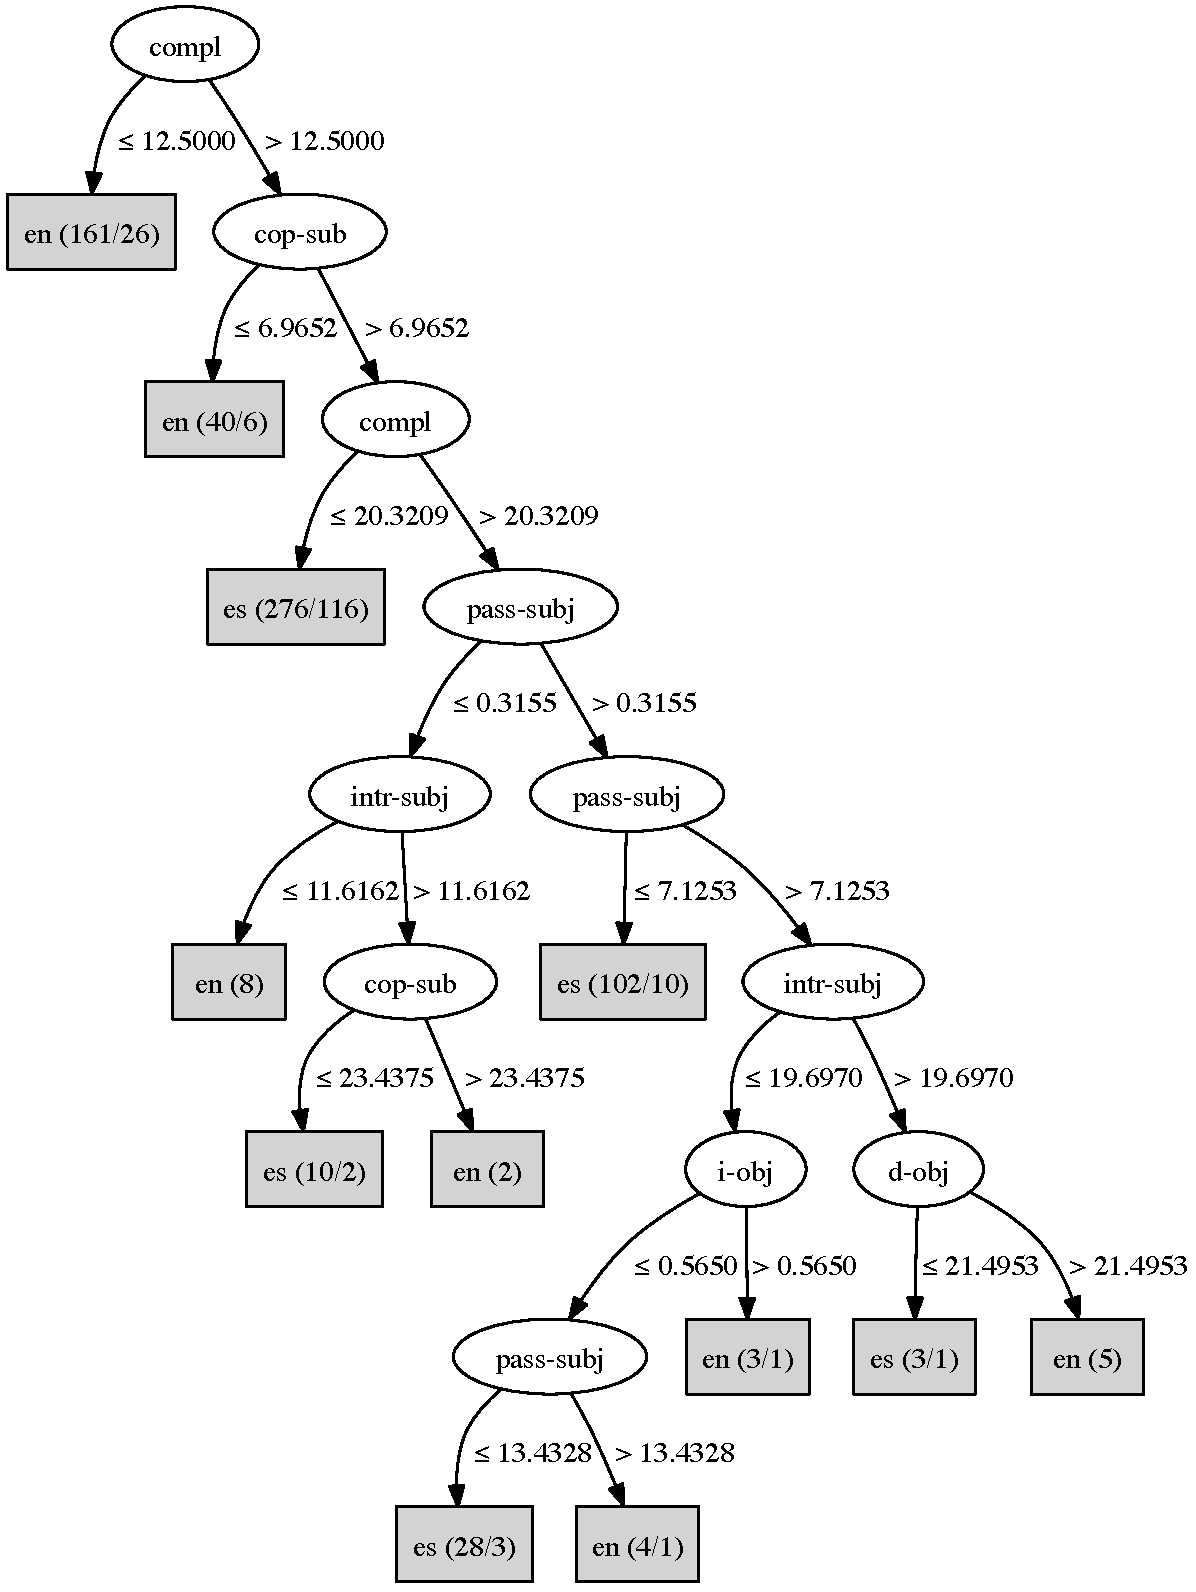
\includegraphics[width=4in]{c45-lex-role.pdf}
\caption{Lexical Argument Role C4.5 Decision Tree}
\label{fig:c4.5-lex-role}
\end{figure}
The other usage of this attribute is in a separate branch, deeper in the tree. Here, using a higher comparison point, low values lead to a branch where the majority are ultimately classified as nonnative, while most high values are classified as native. With these conflicting branches, it is difficult to draw conclusions, but it can be seen that the latter-mentioned branch, the one that appears to coincide with Du Bois's data, does deal with more training cases (43 with 86\% accuracy) than does the other (20 with 90\% accuracy). This suggests that, while a minority of learners overuse lexical intransitive subjects, a large group of learners underuse them. A similar pattern holds with the copular subject. Early in the decision process, one test splits the training cases based on the \textit{cop-sub} attribute and the group with the lower value is immediately classified as native. The other group, which is quite large, undergoes several more tests. The second use of the \textit{cop-sub} attribute is much deeper in the tree and is a direct descendant of the first, meaning that the information content of the attribute was much higher during the first test. This is convenient, as the first test is the one that coincides with Du Bois's data. 

\FloatBarrier
\begin{table}[ht]
\centering
\caption{Accuracy of Lexical Argument Role C4.5 Classifier}
\begin{tabular}{l c c}
\toprule
& Mean & 95\% C.I.\\
\midrule
Nonnative & 78.5\% & - \\
[6pt]Native & 54.8\% & - \\
[6pt]Overall & 66.7\% & 63.0\% --- 70.3\% \\
\bottomrule
\end{tabular}
\label{table:lex-role-results}
\end{table}


The passive subject attribute (\textit{pass-subj}), is used three times in the classifier. The first test that considers it splits off a small number of test cases with low values and passes them on to further tests. This group consists of approximately equal numbers of native and nonnative cases. The other, much larger group is passed onto another test, which also looks at the passive subject attribute. Here, the splitting causes a large number of cases with lower values to be immediately classified as nonnative. Deeper in the tree a pre-terminal node again considers this attribute, and once again classifies low values as nonnative. This is not what one would expect based on Du Bois's data for intransitive subjects. The most likely explanation is that the avoidance of lexical passive subjects by English learners is due to the avoidance of passives altogether. \citet[28.2.3]{butt} note that the passive in Spanish, particularly the form that is exactly parallel to the English passive, employing the copular verb plus a non-finite verb form, is rarely used, and that freedom of word order in Spanish allows simple fronting of an object, which is often why the passive is used in English. It is very likely that this is the source of L1-transfer, resulting in under-usage of the passive, and hence, the lexical passive subject, in learner English.

Du Bois also shows that the direct object role is more likely to be occupied by a NP bearing new information in English than in Spanish. The direct object attribute (\textit{d-obj}) appears once in the decision tree. Cases with low values are immediately classified as nonnative, and those with high values as native. This suggests that L1-interference leads English learners into underusing lexical direct objects. The other two attributes used in the tree, the complement role (\textit{compl}) and the indirect object role (\textit{i-obj}), will not be closely analyzed here owing to a lack of data with which to compare them and to the difficulty of interpretation of their use within the tree.

\subsection{Classification Accuracy}

To gauge the potential accuracy of these attributes in constructing data models for classification, a 10-tree random forest classifier was trained using the lexical argument role attributes (the other attribute sets are too small for use with a random forest classifier). Another such classifier was trained on all 3 attribute sets combined. The results from these classifiers are shown in Tables~\ref{table:lex-role-rf-results} and \ref{table:combined-rf-results}, respectively.
\begin{table}[htbp]
\centering
\caption{Accuracy of Lexical Argument Role Random Forest Classifier}
\begin{tabular}{l c c}
\toprule
& Mean & 95\% C.I.\\
\midrule
Nonnative & 76.6\% & - \\
[6pt]Native & 63.2\% & - \\
[6pt]Overall & 70.0\% & 66.4\% --- 73.5\% \\
\bottomrule
\end{tabular}
\label{table:lex-role-rf-results}
\end{table}
\begin{table}[htbp]
\centering
\caption{Accuracy of Combined Random Forest Classifier}
\begin{tabular}{l c c}
\toprule
& Mean & 95\% C.I.\\
\midrule
Nonnative & 76.6\% & - \\
[6pt]Native & 63.9\% & - \\
[6pt]Overall & 70.2\% & 66.7\% --- 73.8\% \\
\bottomrule
\end{tabular}
\label{table:combined-rf-results}
\end{table}
Considering first Table~\ref{table:lex-role-rf-results}, it does appear that the random forest classifier is able to better take advantage of the data, the average accuracy being boosted from 66.7\% to 70.0\%. However, the overlapping of the confidence intervals means that there is still margin to doubt whether the random forest classifier is better than the C4.5 classifier. Table~\ref{table:combined-rf-results} shows that little is gained by including the other sets of attributes. The valency attributes, as was already shown, are an ineffective basis for classification, and do not seem to improve when combined with other attributes. The failure of the addition of the lexical argument density attributes to improve classification must mean that these attributes do not contribute information that is not already contained in the lexical role arguments.
\newpage
\biblio
\end{document}